\documentclass[compsoc]{IEEEtran}

%%%%%%% USE PACKAGES %%%%%%%
\usepackage{cite}
\usepackage{amsmath, amsfonts, amsthm, amssymb}  % Some math symbols
\usepackage{enumerate}
\usepackage{enumitem}
\usepackage{hyperref}
\usepackage{algorithmic}
\usepackage{graphicx}
\usepackage{textcomp}
\usepackage{xcolor}
\usepackage{natbib}
\usepackage{wrapfig}
\usepackage{changepage}
\usepackage{subfig}
\usepackage{float}
\usepackage{setspace}
\usepackage{hhline}
\usepackage{makecell}
\usepackage[all]{xy}
\usepackage{fancyvrb}
\usepackage[T1]{fontenc}
\usepackage{listings}
\usepackage{fancyhdr}
\usepackage{mathtools}
\usepackage{capt-of}
\usepackage{gensymb}
\usepackage{epstopdf}
\usepackage{booktabs}
\usepackage{centernot}
\usepackage{titlesec}
\usepackage[pdftex]{hyperref}
\usepackage{tocloft}
\usepackage{multirow}
\usepackage{advdate}    % Advancing/saving dates
\usepackage{datetime}   % Dates formatting
\usepackage{datenumber} % Counters for dates
\usepackage[table]{xcolor}
\usepackage{array}
\usepackage{tikz}
\usepackage{pgfgantt}
\usepackage{rotating}
\usepackage[graphicx]{realboxes}
\usepackage{hvfloat}
\usepackage{tcolorbox}
\usepackage{siunitx}
\usepackage{tabularx} 
\usepackage{placeins}

%%%%%%% CONFIGURATION %%%%%%%
\usetikzlibrary{positioning}

\renewcommand{\sfdefault}{ppl}

\pagestyle{fancy}
\fancyhf{}
\renewcommand{\headrulewidth}{0pt}
\cfoot{\thepage}

\DeclarePairedDelimiter{\ceil}{\lceil}{\rceil}
\DeclarePairedDelimiter{\floor}{\lfloor}{\rfloor}
\DeclarePairedDelimiter{\card}{\vert}{\vert}

\usepackage[style=ieee]{biblatex}
\DeclareLanguageMapping{english}{english-apa}
\addbibresource{references.bib}

\def\BibTeX{{\rm B\kern-.05em{\sc i\kern-.025em b}\kern-.08em
    T\kern-.1667em\lower.7ex\hbox{E}\kern-.125emX}}

% \pagestyle{head}
\setlength{\parindent}{0pt}
\setlength{\parskip}{11pt}

%%%%%%% ONE COLUMN %%%%%%% 
\onecolumn
\raggedbottom

%%%%%%% VARIABLES %%%%%%%
\newcommand{\cc}[1]{\texttt{#1}}

\newcommand{\studentOneName}{Aswani, Nishant}
\newcommand{\studentTwoName}{Simsek, Barkin}
\newcommand{\studentOneEmail}{nsa325@nyu.edu}
\newcommand{\studentTwoEmail}{bs3528@nyu.edu}
\newcommand{\advisorOneName}{Karau, Matt}
\newcommand{\advisorTwoName}{Jabari, Saif E.}
\newcommand{\group}{Group 7}

%%%%%%% TUNABLES %%%%%%%
\setlength{\cftbeforesecskip}{7pt}
\setlength{\cftbeforesubsecskip}{7pt}
\setlength{\cftbeforesubsubsecskip}{7pt}

\setcounter{tocdepth}{3}
\hypersetup{colorlinks,linkcolor=,urlcolor=links}

\titlespacing\section{0pt}{12pt plus 4pt minus 2pt}{0pt plus 2pt minus 2pt}
\titlespacing\subsection{0pt}{12pt plus 4pt minus 2pt}{0pt plus 2pt minus 2pt}
\titlespacing\subsubsection{0pt}{12pt plus 4pt minus 2pt}{0pt plus 2pt minus 2pt}

\begin{document}

%%%%%%% COVER PAGE %%%%%%%
\begin{titlepage}

 \begin{center}
 \textbf{\large Senior Capstone Project}
       \vspace*{\fill}

        \textbf {Capstone Final Report\\}
        \textbf {\large ramen: Design and Development of a Raft Consensus Algorithm \\Coupled With a IEEE 802.11 Based Mesh Network for Embedded Systems\\}
        \today
      
        \vfill
            
     \underline {Advisors:}\\
       \advisorOneName\\
       \advisorTwoName\\
       
            
       \vspace{0.8cm}
     
    %   \includegraphics[width=0.4\textwidth]{university}
            
       \underline {\group}\\
       \studentOneName - \studentOneEmail\\
       \studentTwoName - \studentTwoEmail\\
      
            
   \end{center}
\end{titlepage}

%%%%%%% TABLE OF CONTENTS %%%%%%%

\tableofcontents

%%%%%%% TITLE (unused) %%%%%%%%

% \title{\LARGE Design and Development of a Raft Consensus Algorithm Coupled With a IEEE 802.11 Based Mesh Network for Embedded Systems
% \\ 

% {\Large Capstone Fall 2020 Intermediate Report}
% }

% \author{
%     \IEEEauthorblockN{Barkin Simsek}
%     \IEEEauthorblockA{
%         BSc. Computer Engineering
%         \\
%         \textit{bs3528@nyu.edu}
%     }
    
%     \and
    
%     \IEEEauthorblockN{Nishant Aswani}
%     \IEEEauthorblockA{
%       BSc. Computer Engineering
%         \\
%         \textit{nsa325@nyu.edu}
%     }
% }

\newpage
\setstretch{1.25}

%%%%%%% ABSTRACT %%%%%%%
\section{Abstract}
% Used to indicate where a new paragraph starts within the abstract 
\newcommand{\nextInternalParagraphStartsHere}{}

Consensus is a fundamental problem in fault-tolerant distributed systems and involves multiple nodes arriving at a coordinated decision. Reaching a consensus is more challenging if the system is dynamic and in real-time, as is the case with autonomous vehicles and mobile sensor networks. Thus, consensus algorithms ensure that a cluster of devices can cooperatively complete a mission even if the cluster loses its leader. However, if a consensus algorithm is built upon a typical hub-spoke network topology, the algorithm may be rendered useless if the singular network access point fails. \nextInternalParagraphStartsHere A mesh network is an alternative, non-hierarchical topology for local networks in which devices can directly communicate amongst themselves without a central network traffic controller. As a result, a mesh network is resilient to a single point of failure. \nextInternalParagraphStartsHere Our capstone project aims to implement Raft, a distributed consensus algorithm, atop a mesh network for use in low-power embedded systems. An open-source software library will be developed and prototyped on a printed-circuit board (PCB) with an ESP8266 chip. 


%%%%%%% BACKGROUND RESEARCH %%%%%%%

\section{Background Research}
%%%%%%%%%%%%%%%%%%%%%%%%%%%%%%% Introduction %%%%%%%%%%%%%%%%%%%%%%%%%%%%%%%%%%%%

As of 2020, more than 50 billion devices are estimated to be using IEEE 802.11 based WiFi radios due to its low cost, robustness, and ease of use. \cite{G_Davis_2018}. The IEEE 802.11 standard, ratified in 1997, is a set of protocols for wireless communication to standardize the use of Wireless Local Area Networks (WLANs) \cite{perahia2013next}. This standardization, combined with the formation of the WiFi alliance and reduction in technological costs, led to the rapid adoption of wireless communication throughout the 2000s \cite{perahia2013next}. 802.11 made internet mobility a reality for everybody, proliferating the use of mobile technologies and paving the path for the future of communication. 

%%%%%%%%%%%%%%%%%%%%%%%%%%%%% Why mesh networking %%%%%%%%%%%%%%%%%%%%%%%%%%%%%%%%
% resilience and low power consumption emphasis

Since then, wireless communication has been evolving. Cars, drones, and traffic lights, to name a few, are all able to communicate wirelessly, each able to afford their own network requirements. Networks can be classified by their topologies, which refers to the arrangement of the nodes in the network. Among others, exist the hub-spoke and the mesh topologies. Used in Wi-Fi, the hub-spoke topology implies the existence of a central access point (AP) that acts as the gateway for all traffic within and beyond the local network \cite{ti_lethaby2017wireless}. On the other hand, a mesh network is where all devices are able to inter-communicate without the presence of a central node to organize traffic \cite{ti_lethaby2017wireless}. In mesh networks, any node(s) can act as an internet gateway \cite{ti_lethaby2017wireless}. 

\begingroup
    \centering
    \medskip
    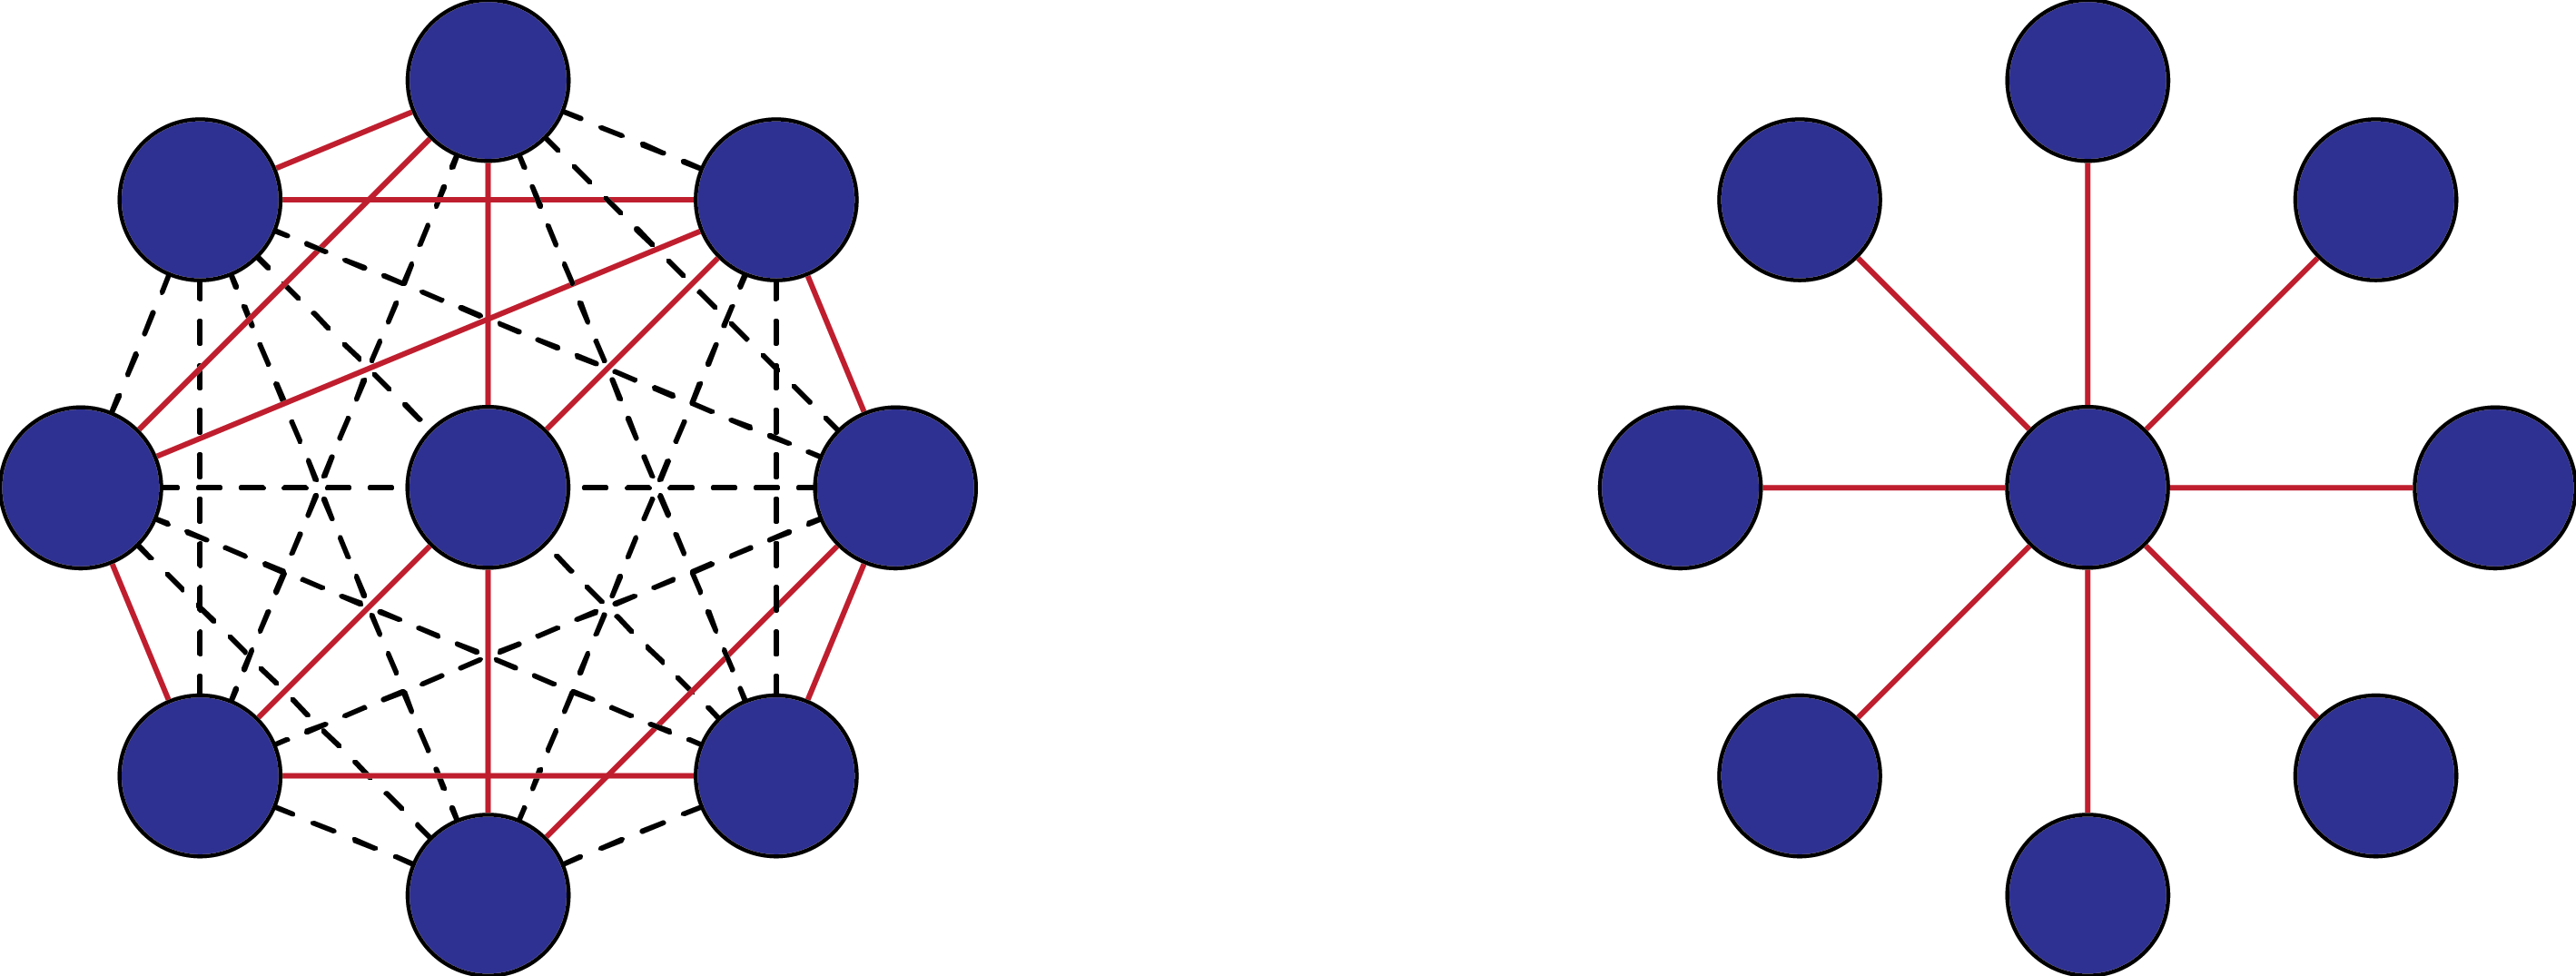
\includegraphics[width=0.5\columnwidth]{final-proposal/images/mesh_vs_hub_spoke.png}
    \captionof{figure}{Left: A mesh network topology, Right: A hub-spoke network topology}
    \label{fig:consensus_mesh}
\endgroup

While a hub-spoke topology is sufficient for most typical applications, certain use cases require the resilience a mesh network provides. In the case of group robotics, "centralized systems [...] require a lot of computer performance from the commander" \cite{manet_drone_semenova2015network}. On the other hand, a mesh topology is "less prone to failure" \cite{manet_drone_semenova2015network} and allows for greater independence of each node. Similarly, vehicular networks require the consideration of a "highly dynamic topology" \cite{iov_wu2016internet} where nodes are moving at high speeds but also have "high reliability requirements" \cite{iov_wu2016internet} due to safety concerns, making mesh topologies an ideal choice. 


%%%%%%%%%%%%%%%%%%%%%%%%%%%%% Why consensus algorithms %%%%%%%%%%%%%%%%%%%%%%%%%%%%
% resilience and dynamic topology emphasis

However, in order to meaningfully complete a task, these groups of autonomous devices must be able to coordinate and come to an agreement, or a consensus. The topic of consensus is a challenging problem in distributed systems aimed at arriving at a collective agreement across all the nodes in a system, even in the presence of malfunctioning nodes \cite{Bach_Mihaljevic_Zagar_2018}. The \textit{Byzantine Generals Problem} proposed by \textit{L. Lamport} in 1982 is an analogy that helps visualize the need for such algorithms \cite{Lamport_1983}. According to the \textit{Byzantine Generals Problem}, a Byzantine army wants to attack a fort. As a result, each Byzantine general must decide whether to attack the target fort or retreat for protection. The caveat is that all of the generals must perform the same action at the same time in order to minimize the number of losses. However, the generals are located very far apart from each other and can only communicate through designated messengers, who may be lost or captured during their mission. Thus, the generals need to find a reliable way to exchange messages and reach a consensus in order to be successful. 

Consensus algorithms ensure that the critical information is reliably replicated for each node (or "generals" in the \textit{Byzantine Generals Problem}) within a system \cite{tsitsiklis1984problems}. Consensus algorithms also ensure that the nodes within the system can work as a team and succeed in their mission even if some of the nodes fail and the network topology changes \cite{raft_paper}. Therefore, consensus algorithms play a crucial role in managing a group of nodes autonomously and provide resilience against threats, external or internal \cite{Kar_Moura_2010}. Additionally, consensus algorithms provide the flexibility to add new nodes to the network, as needed, since nodes with the network can rearrange themselves autonomously \cite{Olfati_Saber_Fax_Murray_2007}. 

Similar to the \textit{Byzantine Generals Problem}, in today's world, interconnected embedded and IoT devices often need to reach a consensus in order to perform required tasks successfully and efficiently \cite{Orostica_Nunez_2019}. For example, a group of drones tasked to survey a specific area could be preprogrammed individually to complete the task. However, having connectivity and consensus between these drones could drastically increase their efficiency and success rate by dynamically updating their routes based on the new information available. In the event of a drone loss, the remaining drones could communicate this information, and a specific drone could take over additional tasks. Furthermore, new drones could easily be added to the group as needed since the consensus can rearrange itself. 

%%%%% Combining consensus algorithms and mesh networking and embedded devices %%%%% 
% Challenge of addressing problem

\begingroup
    \centering
    \medskip
    
\includegraphics[width=0.5\columnwidth]{final-proposal/images/consensus_traditional.png}
    \captionof{figure}{A consensus algorithm implemented on top of a hub-spoke network topology}
    \label{fig:consensus_traditional}
\endgroup

A consensus algorithm could be implemented on top of traditional hub-spoke network topology, as shown in Figure \ref{fig:consensus_traditional}. The blue circles in the diagram represent the member nodes within the system, and the green circle represents the leader node. Since a hub-spoke topology is used, the green circle also represents the "hub" node in the network topology, where all of the connections meet and redistribute. A consensus algorithm implemented in this way would work without issues until there are any problems with the leader node. Even though consensus algorithms are capable of electing new leaders \cite{raft_paper}, the consensus algorithm would fail when the "hub" node fails in a hub-spoke network topology. This is the case because the member nodes in the system would not be able to communicate with each other and perform a leader election. Therefore, consensus algorithms implemented on hub-spoke network topologies are prone to a single point of failure. If we think about the previously given drone example, if the "hub" drone fails during the mission, the rest of the team would not be able to communicate with each other and reach a consensus.

\begingroup
    \centering
    \medskip
    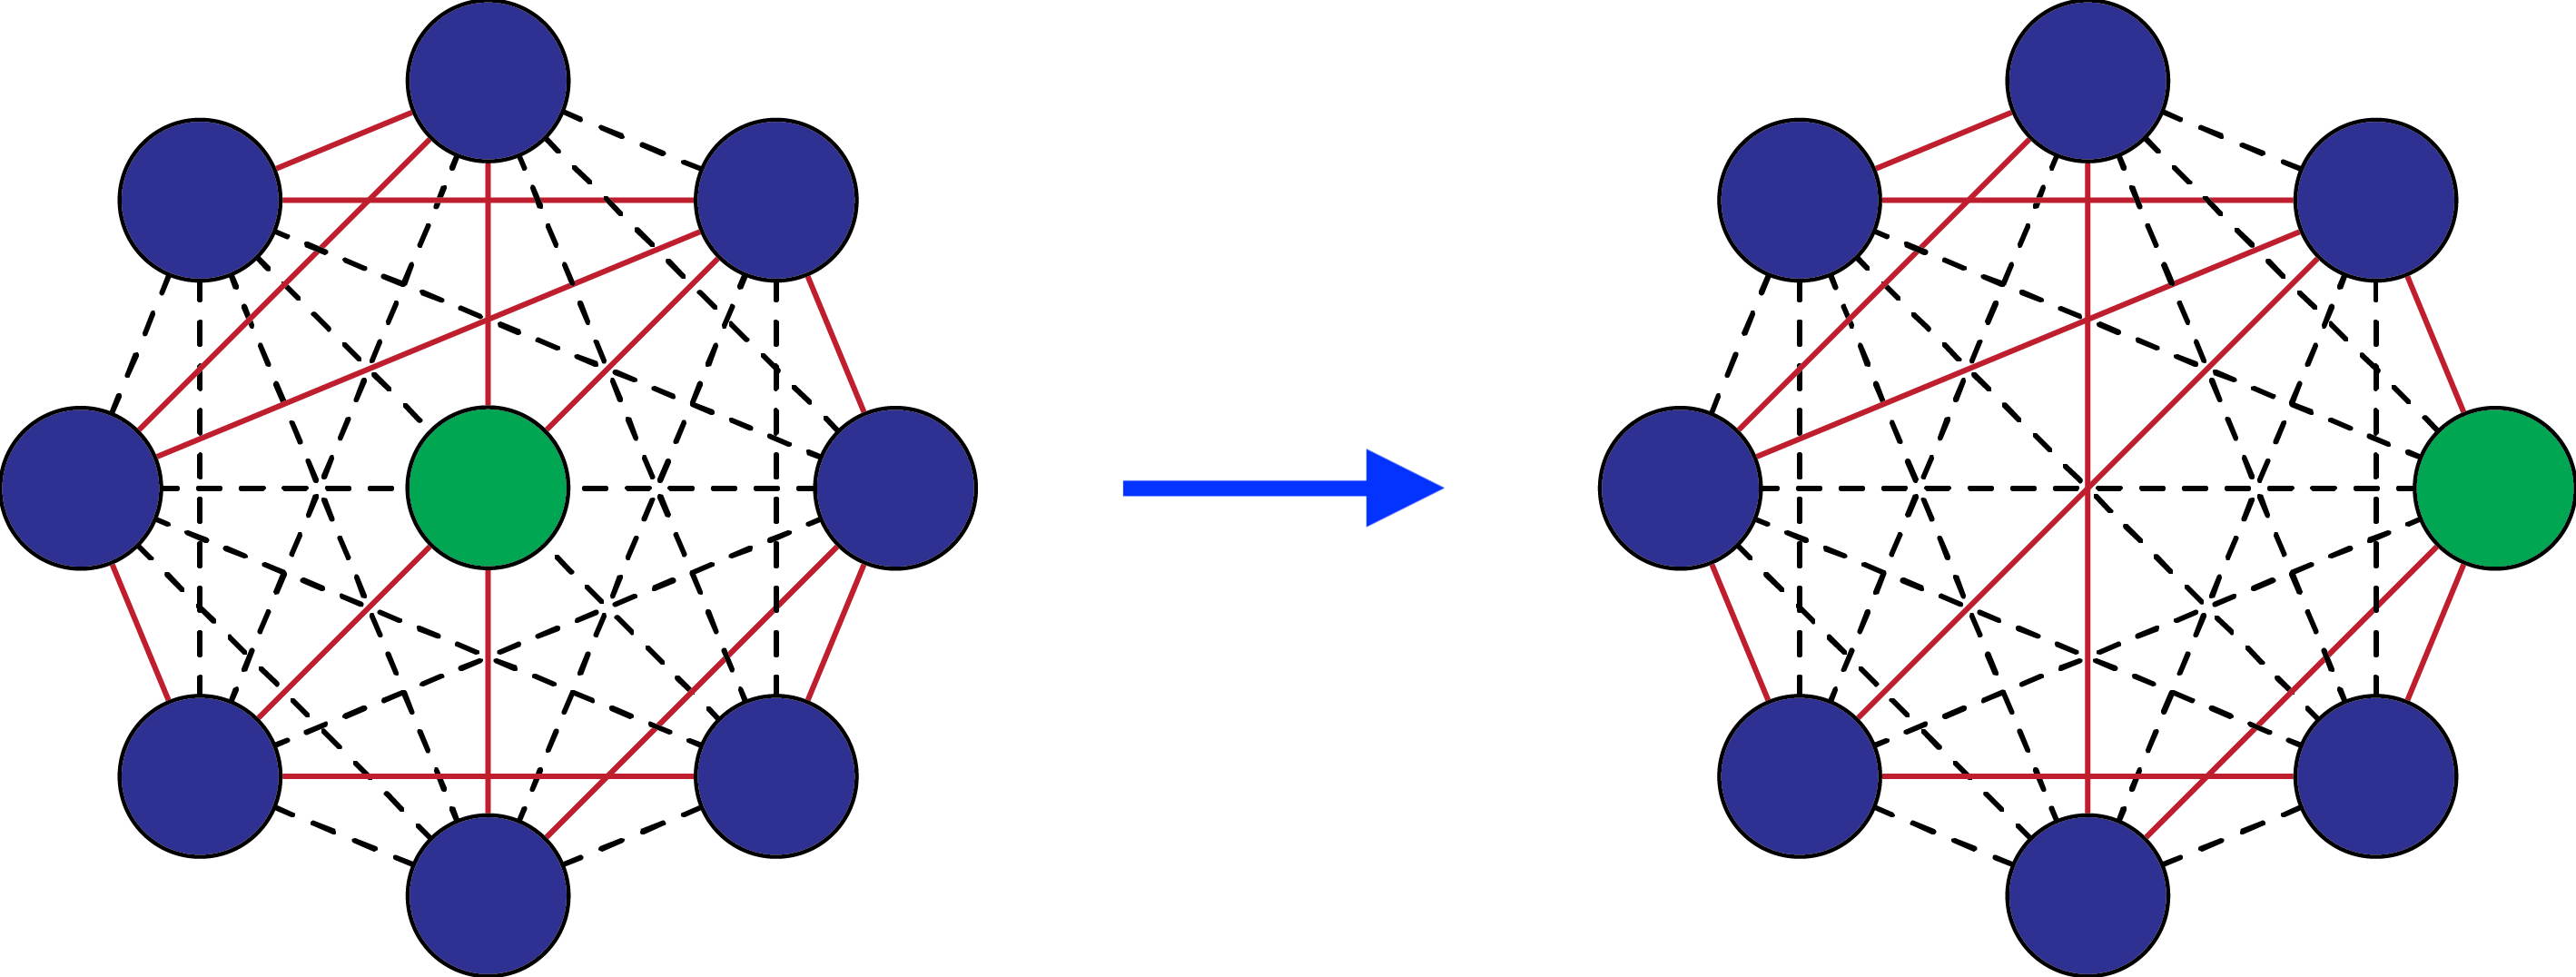
\includegraphics[width=0.5\columnwidth]{final-proposal/images/consensus_mesh.png}
    \captionof{figure}{A consensus algorithm implemented on top of a mesh network topology}
    \label{fig:consensus_mesh}
\endgroup

Consensus algorithms could also be implemented on top of a mesh network topology, as shown in Figure \ref{fig:consensus_mesh}. The blue circles once again represent the member nodes, and the green circle represents the leader node. However, as opposed to the implementation shown in Figure \ref{fig:consensus_traditional}, every member code can connect to each other without a need for a "hub" node. Thus, even if the leader node fails, the remaining nodes can elect a new leader node and reach a consensus. There is no single point of failure in the system shown in Figure \ref{fig:consensus_mesh}, and this situation significantly increases a system's resilience and flexibility. In light of these insights, our capstone project aims to combine mesh networking with consensus algorithms.

%%%%%%% PROBLEM DEFINITION %%%%%%%
\section{Problem Definition}
\subsection{Problem Analysis}
In order to clarify the scope of the problem, the 5W method was used:

\begin{enumerate}

    \item Who has the problem?
    \begin{enumerate}
        \item Groups of mobile machines (drones, cars, rovers) with embedded systems that are tasked to achieve a mission autonomously
    \end{enumerate}
    
    \item What is the problem?
    \begin{enumerate}
        \item In certain cases, these autonomous devices may fail to complete a mission or a set of tasks due to communication issues amongst themselves when using a hub-spoke system.
    \end{enumerate}
    
    \item Where does the problem occur?
    \begin{enumerate}
        \item The problem can occur in geographies where stable communication between devices connection is not possible or where the devices are not easily accessible to service by humans.
    \end{enumerate}
    
    \item When does the problem occur?
    \begin{enumerate}
        \item The problem can occur at any given moment. It has to do with the leader or a hub node failing within the hub-spoke topology.
    \end{enumerate}
    
    \item Why does the problem occur?
    \begin{enumerate}
        \item The problem occurs because all traffic is routed through these leader or hub nodes. Hence, if this node fails, communication also fails because other nodes are not able to organize themselves anymore.
    \end{enumerate}
\end{enumerate}


\subsection{Problem Clarification}
%   Problem Clarification
    % Black-box model
%%%%%%% %%%%%%% %%%%%%% 

%The main objective of this capstone is to develop a consensus algorithm coupled with a mesh network topology. 

The black-box model of this monitoring system can be seen in Figure \ref{fig:black_box}. The sensors on a node will be collecting data, which will then be fed to the decision logic, implemented in the form of a consensus algorithm. Each of these nodes will be communicating with one-another using a Wifi-based mesh network and updating their logs as a result of this communication. Eventually, each of the nodes will then carry out some actuation or state indication.

As there are multiple implementations of an 802.11 based mesh network, it is out of the scope of this project to be able to interface with all of them. Our implementation will focus on what is readily available and will be designed in a way so that with minimal future development, another implementation of a mesh network could replace the one we use.

There are also quite a few options for consensus algorithms. However, our system will be limited to a single consensus algorithm, namely Raft \cite{raft_paper}. Section \ref{conceptualization_consensus} describes the reasoning behind selecting Raft.

\begingroup
    \centering
    \medskip
    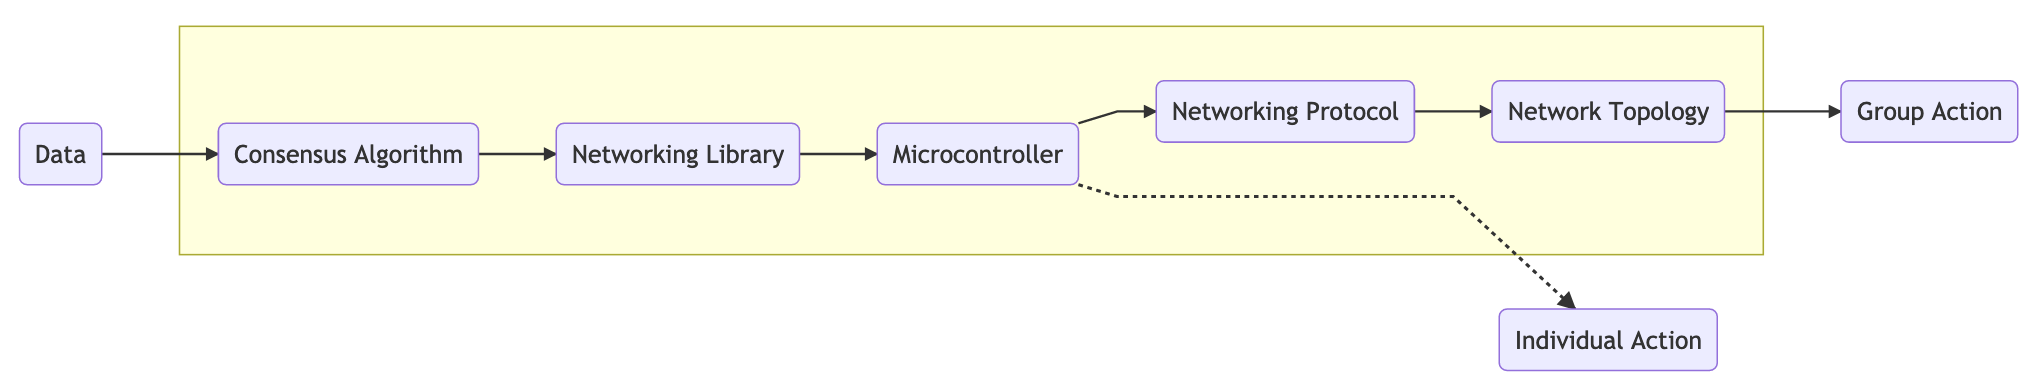
\includegraphics[width=0.95\columnwidth]{final-proposal/images/blackbox.png}
    \captionof{figure}{A black box diagram for each node of the system}
    \label{fig:black_box}
\endgroup

\subsubsection{Networking Protocols}
There are a plethora of network types for communication between industrial nodes, such as control area networks (CAN), Profibus, and Modbus \cite{lee2007comparative}. However, wired communications limit the flexibility of the nodes attached, especially in cases where these nodes are mobile. Hence, we turn to wireless networks, where there are four dominant protocols: Bluetooth, Ultra-wideband (UWB), Zigbee, LoRa, and Wifi \cite{lee2007comparative, ti_lethaby2017wireless}.

Mesh networks are not limited to any one of these standards. In fact, "IoT-related wireless technologies [...] are extremely heterogeneous in terms of protocols, performance, reliability, latency, cost effectiveness, and coverage",  \cite{iot_survey_cilfone2019wireless}. Each standard has its niche of operation: IoT devices may employ the IEEE 802.15.4 standard or Bluetooth for short-range communications, whereas mid to long-range communications may make use of IEEE 802.11, which was amended in 2011 to support mesh networks \cite{ti_lethaby2017wireless, iot_survey_cilfone2019wireless}. Figure \ref{fig:comparison_protocols} shows a comparative performance analysis of LoRa, Zigbee, Wifi, and Bluetooth, highlighting how each protocol has its strengths and weaknesses.

\begingroup
    \centering
    \medskip
    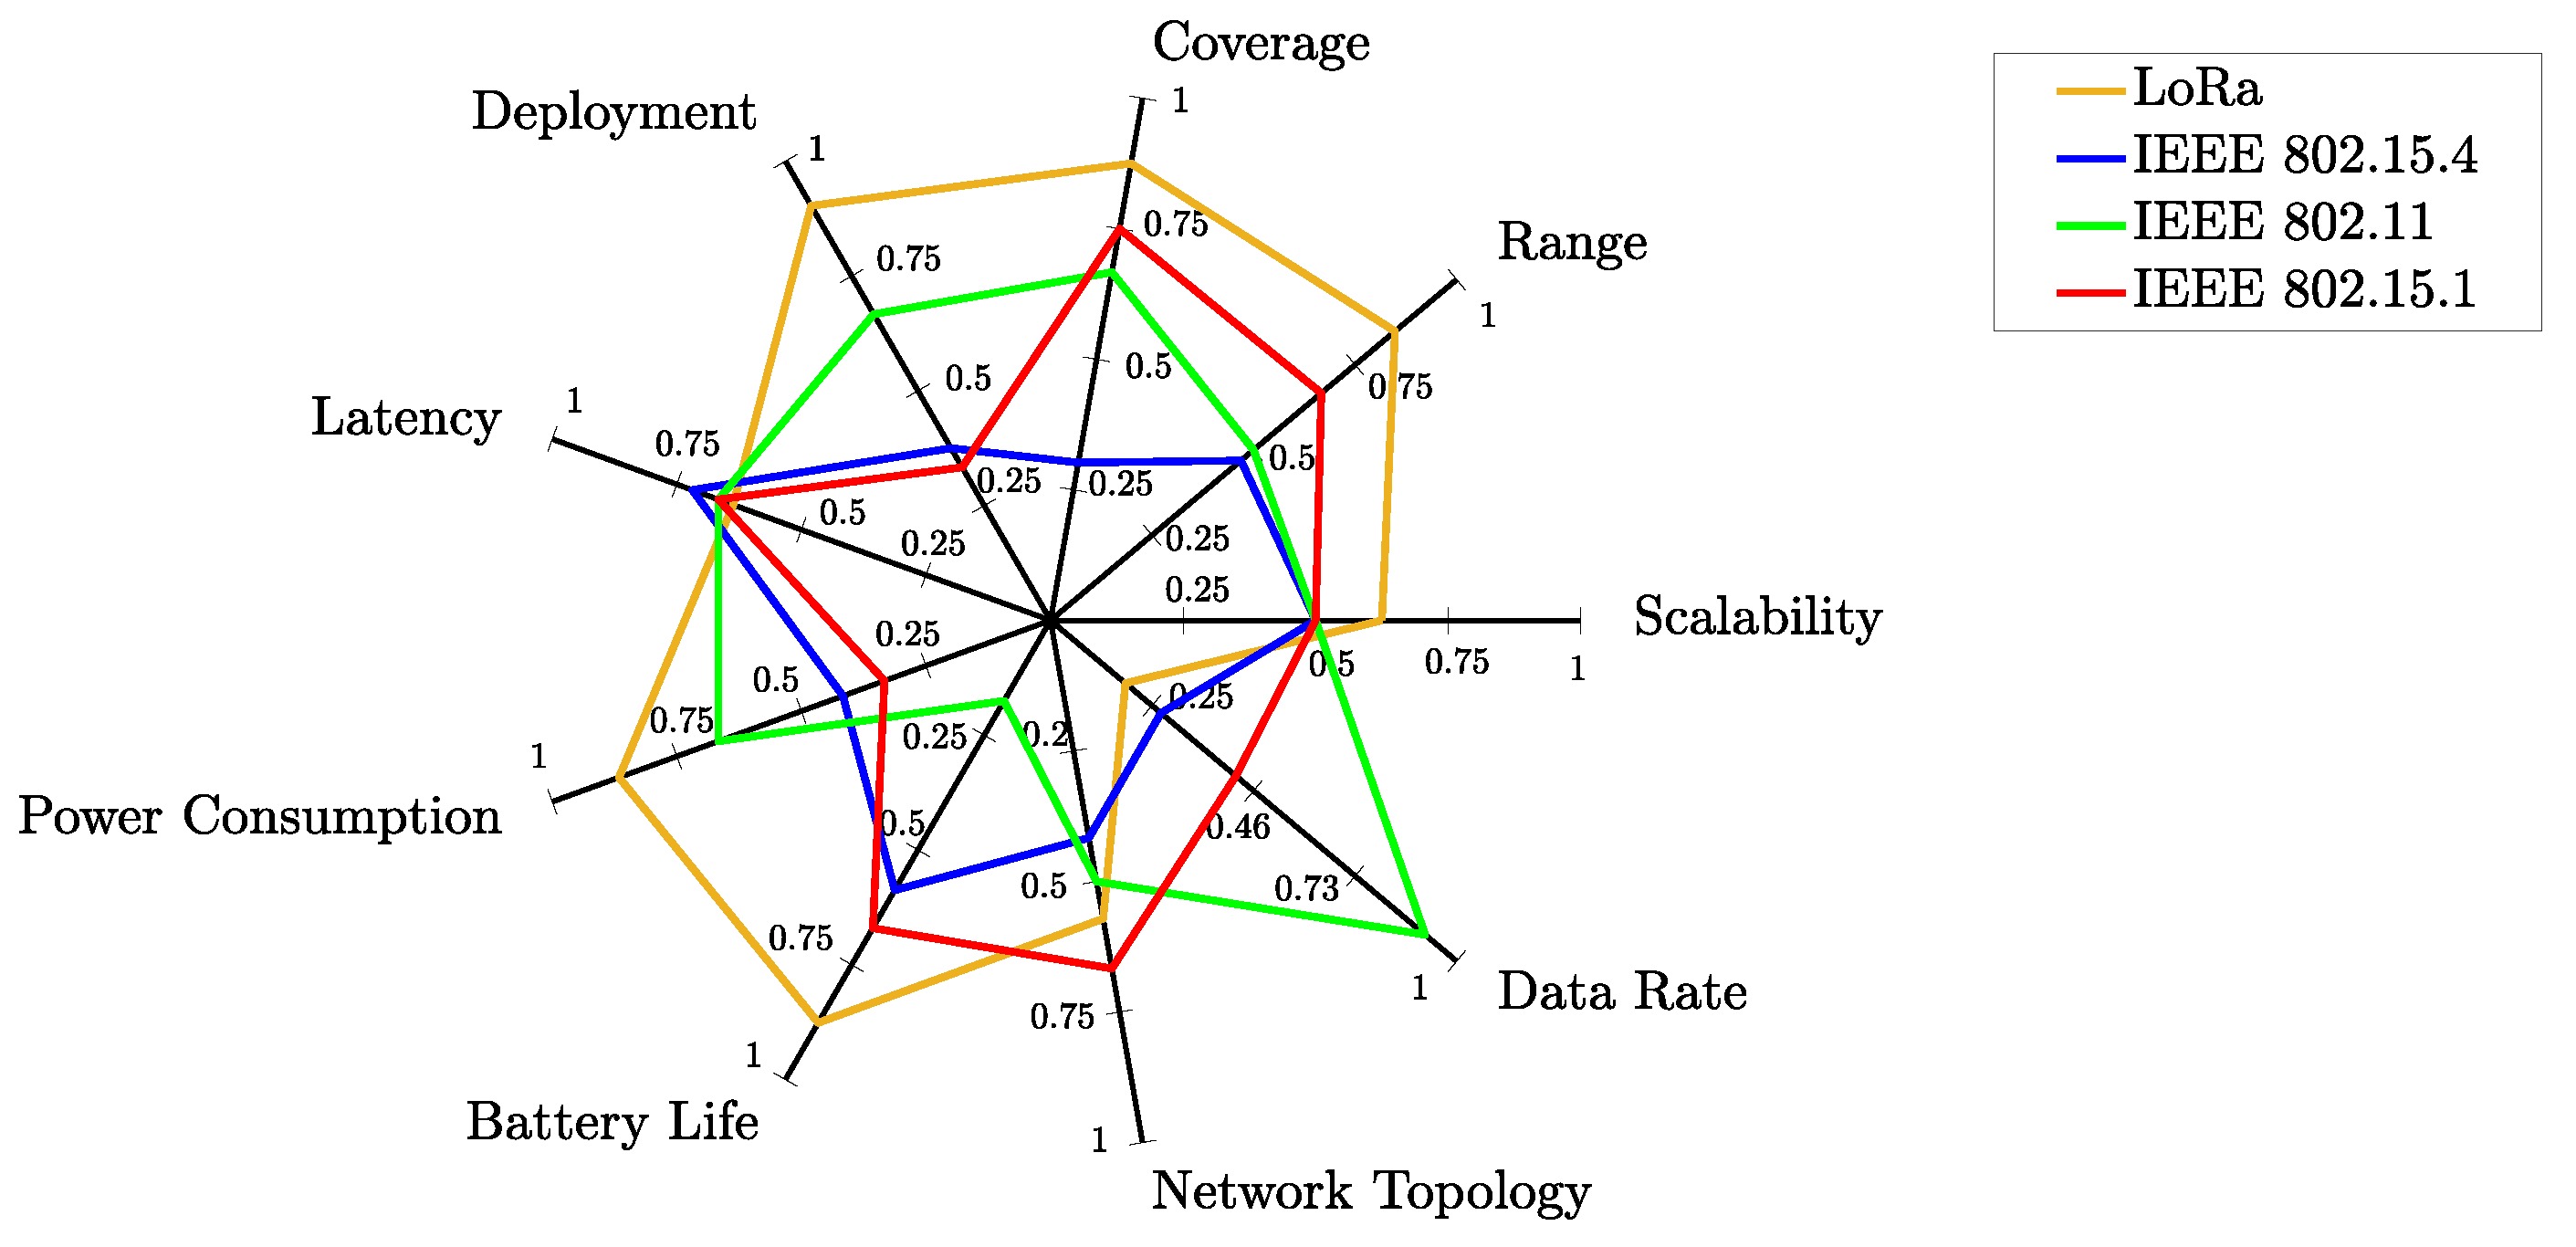
\includegraphics[width=0.85\columnwidth]{final-proposal/images/comp_perf_analysis.png}
    \captionof{figure}{Comparative performance analysis of four protocols. \\Source: Adapted from \cite{iot_survey_cilfone2019wireless}}
    \label{fig:comparison_protocols}
\endgroup

While the implementation of mesh networks and consensus algorithms are agnostic to the protocol underneath, it is important to address these concepts in the context of real-world constraints. Current IoT research "assumes that the devices are equipped with low-power IEEE 802.15.4 (Zigbee) transceivers" \cite{disney_glaropoulos2013enhanced}. Yet, a significant portion of deployed embedded systems and consumer electronics carry IEEE 802.11 compatible hardware \cite{disney_glaropoulos2013enhanced}. 
The "wide penetration of IEEE 802.11" \cite{disney_glaropoulos2013enhanced} then makes it the more attractive choice because hardware does not need to be redeployed to support newer standards. Despite 802.11's notoriety as a high power consumer, research indicates that additional firmware controlling the sleep scheduling can help lead to significant energy savings \cite{disney_glaropoulos2013enhanced, barghi2019practicalpower}

Furthermore, 802.11 has built-in support for mesh networks as a result of the 802.11s amendment. The amendment describes mesh stations (mesh STAs) and their ability to link with one another without the requirement of a central AP; rather, certain nodes may act as mesh access points (MAP) to connect to another network \cite{iov_wu2016internet, optical_zeitgeist_laboratory_2011}.

Given 802.11's ubiquity and built-in support for mesh networks, we found it fit to work with an 802.11-based network.

\subsubsection{Consensus Algorithms}
\label{conceptualization_consensus}
With the rapid increase in adoption and development of distributed \& multi-agent systems, achieving a consensus across these systems became an important issue because of the high potential for scalibility \cite{Ge_Han_Ding_Zhang_Ning_2018}. Achieving consensus across such systems allow autonomous air vehicles, cooperative IoT devices, sensor networks to be built at a scale. 

The distributed consensus algorithms can be classified into three categories based on their hierarchical structure: \emph{leaderless consensus algorithms}, \emph{leader-following consensus algorithms}, and \emph{containment control algorithms} \cite{consensus_systems_survey}. In \emph{leaderless consensus algorithms}, there are no leaders and the nodes within the system are expected to asynchronously converge on a target \cite{Ge_Han_2017}. However, in \emph{leader-following consensus algorithms}, there is a leader node that orchestrates the actions of the rest of the network. Finally, in \emph{containment control algorithms}, there might be more than one leader to orchestrate different types of operations within the system. A visualization of the different types of consensus algorithms can be seen in Figure \ref{fig:consensus_types_detailed}, where green circles are the leaders in the system and orange lines represent the logical connections between the consensus members.

\begingroup
    \centering
    \medskip
    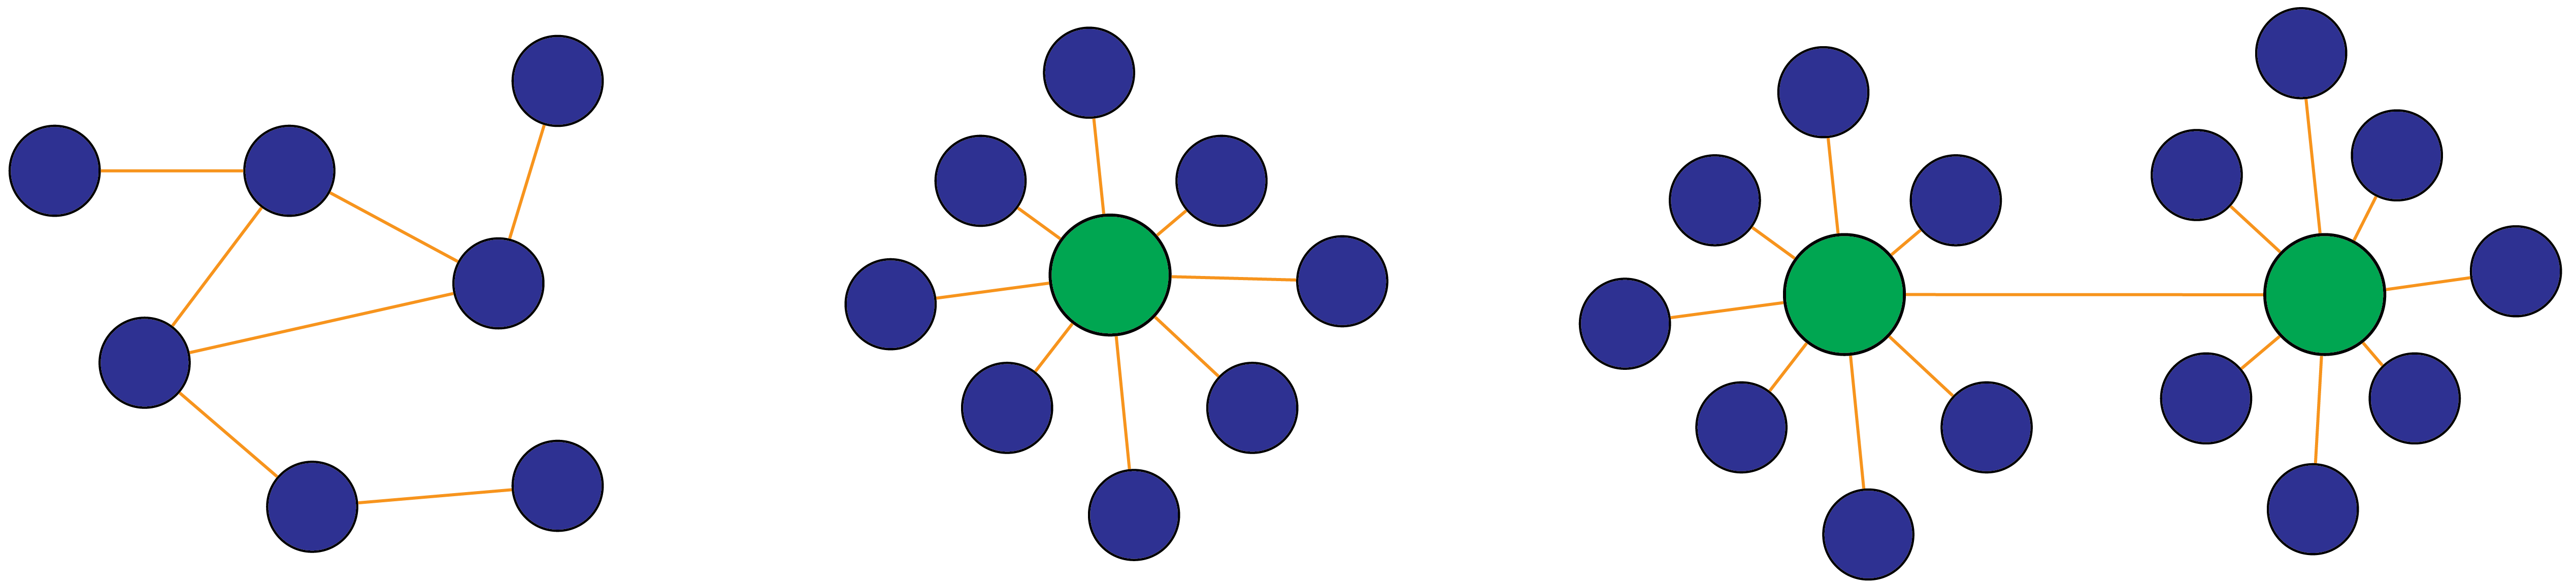
\includegraphics[width=0.75\columnwidth]{final-proposal/images/consensus_types.png}
    \captionof{figure}{Left: A leaderless consensus algorithm, Middle: A leader-following consensus algorithm, Right: A containment control algorithm}
    \label{fig:consensus_types_detailed}
\endgroup

The distributed consensus algorithms can also be classified into two categories based on when they transfer information to reach a consensus: \emph{time-triggered consensus algorithms} and \emph{event-triggered consensus algorithms} \cite{consensus_systems_survey}. In \emph{time-triggered consensus algorithms}, the nodes in the system initiate the information transfer once a set amount of time elapses. Additionally, if the consensus algorithm is asynchronous by design, each node can have a randomly set time duration before they send information. On the other hand, in \emph{event-triggered consensus algorithms}, the nodes in the system initiate information transfer when an external event occurs. A visualization of the different types of consensus algorithms can be seen in Figure \ref{fig:consensus_time_based_and_evevent_based}, where orange circles represent the timer of the nodes, green arrow represents the external event trigger, and red arrows represent the information transfer.

\begingroup
    \centering
    \medskip
    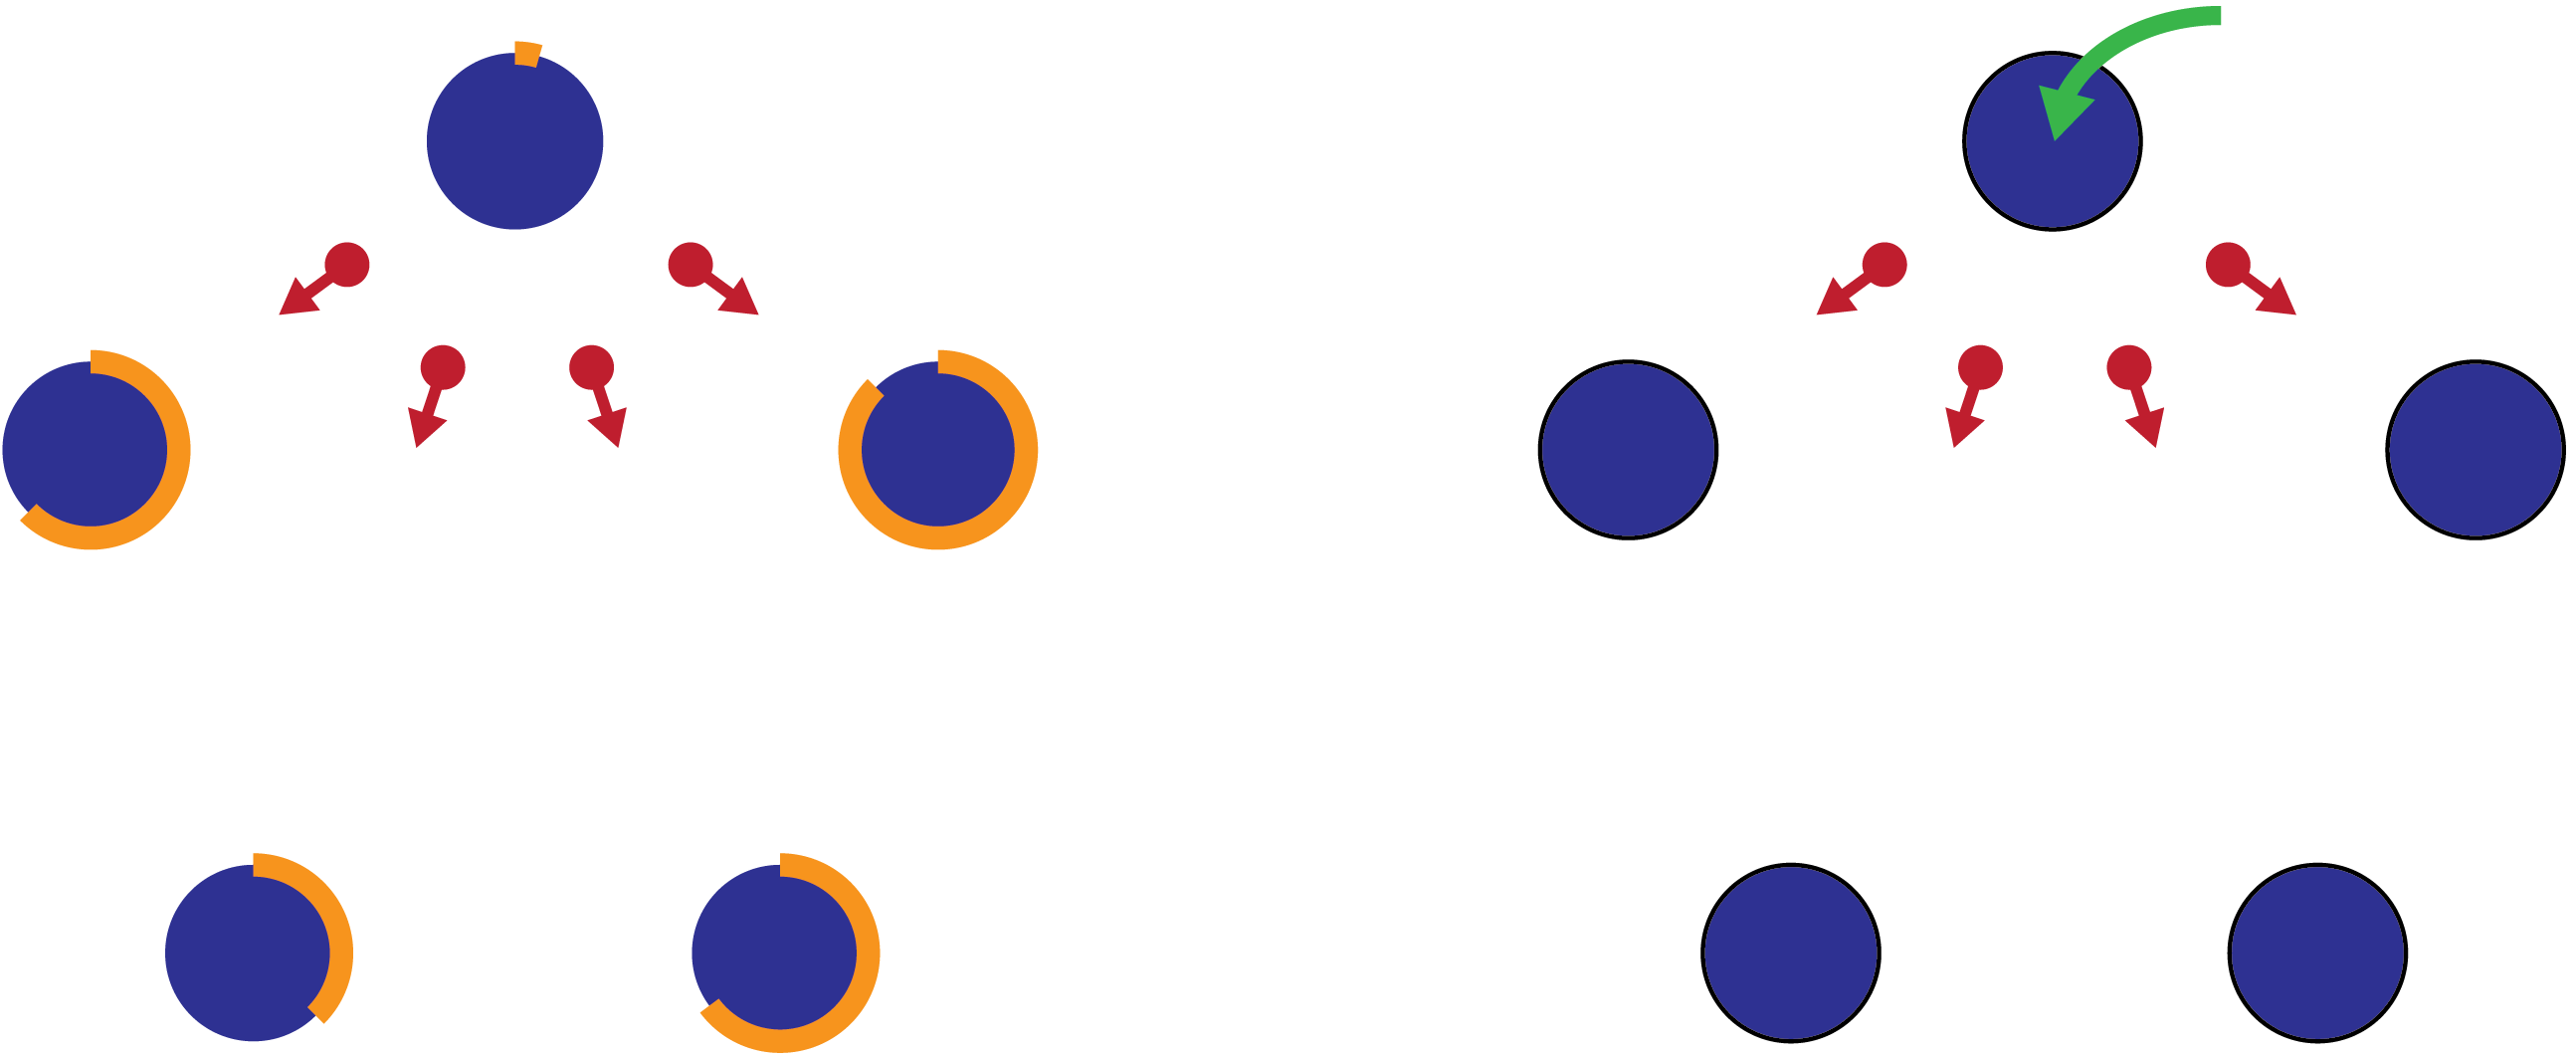
\includegraphics[width=0.45\columnwidth]{final-proposal/images/consensus_time_based_and_evevent_based.png}
    \captionof{figure}{Left: A time-triggered consensus algorithm exchanging messages when the timer goes off, Right: An event-triggered consensus algorithm exchanging messages when an event occurs (green arrow)}
    \label{fig:consensus_time_based_and_evevent_based}
\endgroup

Paxos and Raft are among the most popular \& practical distributed \emph{time-triggered} and \emph{leader-following} consensus algorithms available \cite{paxos_vs_raft}. Paxos has been the industry's first choice since it was published even though the way it works is not intuitive and difficult to understand. Since the Raft consensus algorithm aims to be simple and easy to understand \cite{raft_paper}, it is gaining more and more popularity in the industry. Furthermore, the Raft consensus algorithm aims to abstract the way the underlying technology works and not make it specific to a system \cite{paxos_vs_raft}. As a result, the Raft consensus algorithm is more suitable for experimenting and implementing on non-traditional topologies like mesh networks.

\subsubsection{Microprocessors}
Microcontroller units (MCUs) are a hefty consideration for any IoT solution. Unsurprisingly, there is a large variety of MCUs at different levels of "memory, power, computational capability, architecture etc." \cite{bansal2020iotsurveydevices} for various applications. These devices sit at different levels of the IoT ecosystem, implying that not all devices are required to be homogeneous in their capabilities. For discussion purposes, we adopt the classification system described in Bansal & Kumar's survey of IoT technologies \cite{bansal2020iotsurveydevices}. Class 0 devices may have 1-50KB of RAM with clock speeds below 100MHz, class 1 devices range from 100KB-100MB of RAM with clock speeds between 100MHz-1.5Ghz, and class 2 devices generally have resources greater than those of class 1 \cite{bansal2020iotsurveydevices}. Generally speaking class 0 devices such as the TELOSB are employed for Wireless Sensor Network (WSN) use-cases to collect data and perhaps perform simple actuation. On the other hand, class 1 devices, such as the well-known Raspberry Pis, are more suitable for coordination, media processing, data filtering tasks, etc.

Given our design constraints, namely dynamic topology and decision making capabilities, we would expect this system to work with embedded systems on mobile technologies such as drones, vehicles, and rovers. While such devices are often fitted with class 2 devices, the goal of our project is to be able to deploy such a networking ability on class 1 devices as well. Espressif's ESP8266 chip stands out as an option: the chip is designed to be a Wifi chip with a focus on low-cost and minimal peripherals. The MCU operates between 80-160MHz and has 50KB of SRAM with up to 16MB of external flash memory \cite{espressif:esp8266}, so it is on the lower-end of the class 1 category. Moreover, there is a decent open-source community dedicated to the MCU and Espressif has released a mesh networking software development kit (SDK) for its chips with detailed documentation \cite{esp-mesh-docs}. 


\subsection{Problem Statement}
%   Problem Statement
    % Clarify the scope of the problem [kinda done]
    % Project Aim [done]
%%%%%%% %%%%%%% %%%%%%% 

The of this Capstone Project is to design and develop a resilient wireless mesh network architecture coupled with a consensus algorithm for low-power embedded devices in dynamic topologies, demonstrated using 802.11-based ESP8266 boards.

We aim to create an open-source software library that anybody could incorporate in a system which requires nodes to work autonomoulsy together. We plan to demonstrate our software library through prototype boards that will each consist of an ESP8266 MCU, power sensors, and LEDs. Our software library will be installed on these boards to enable them to form a mesh network and run the Raft consensus algorithm. We will show how a signal propagates in the Raft consensus algorithm within the mesh network using LED lights as shown in Figure \ref{fig:mesh_signal_propagation}. We will also demonstrate how the network can realign \& recover itself by turning on and off randomly selected ESP8266 microchips.

\begingroup
    \centering
    \medskip
    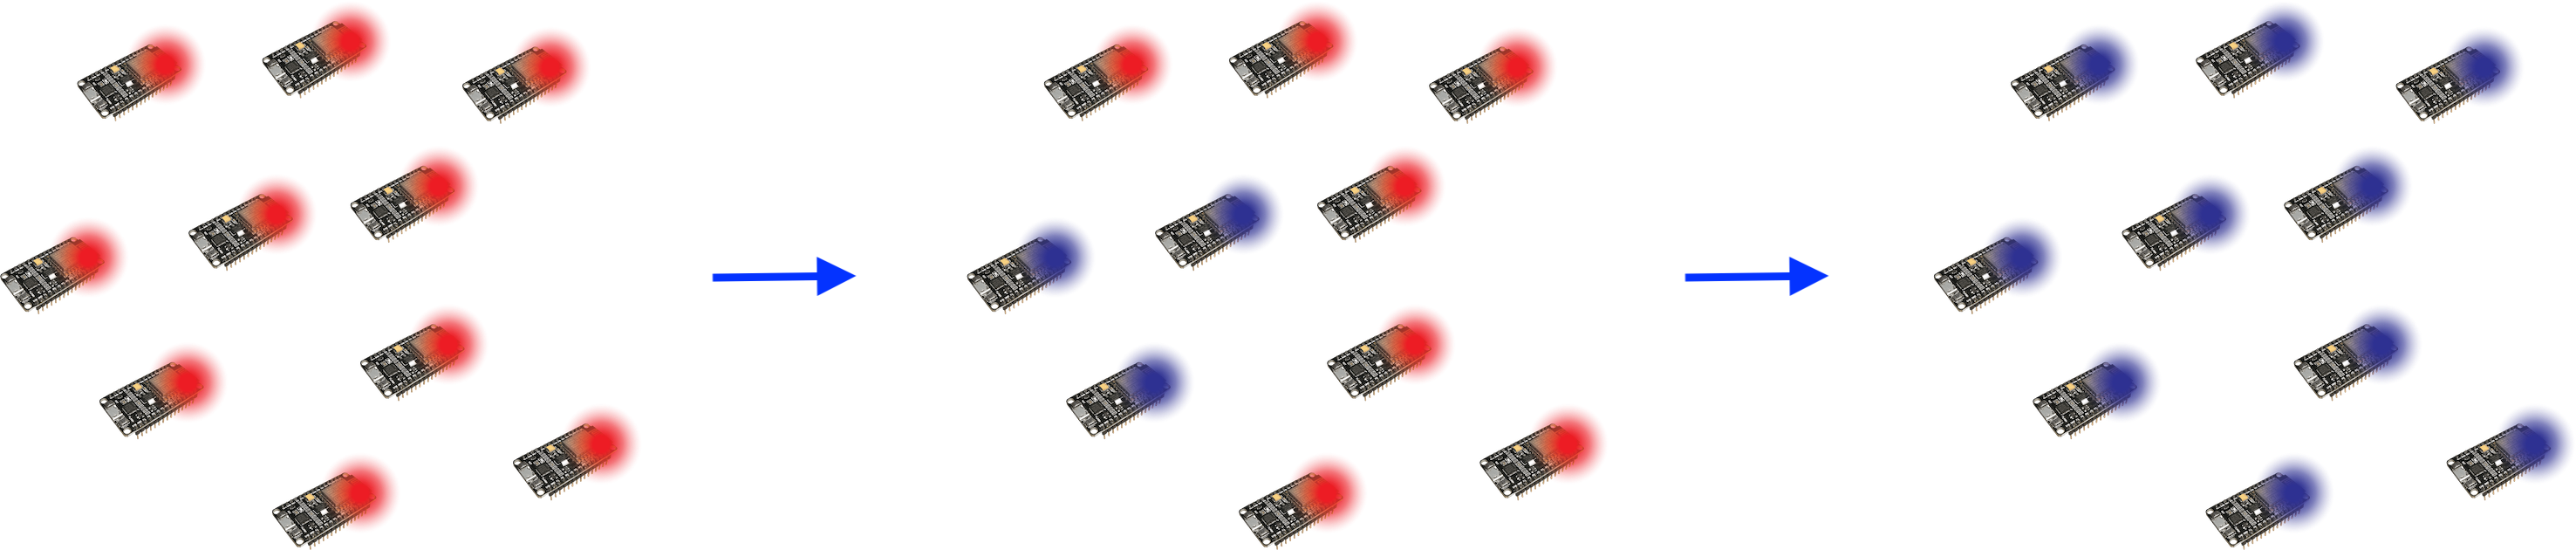
\includegraphics[width=\columnwidth]{final-proposal/images/mesh_signal_propagation.png}
    \captionof{figure}{An ESP8266 cluster transitioning to the blue state from the red state using our software library. Red and blue LEDs are used to represent the states.}
    \label{fig:mesh_signal_propagation}
\endgroup

%%%%%%% DESIGN CONSTRAINTS %%%%%%%
\section{Design Constraints}
\subsection{Technical}

Taking into account market demands, history of the topic, and potential applications, there are various technical constraints on our system:

\textit{Resilient to threats:} Similar to managing a dynamic topology, the system should also be resilient to handling abrupt changes to the system to ensure that the task is distributed. The final design aims to recover from the loss of a leader within 1000\si{\ms}.

\textit{Scalability:} The system should be able to reasonably perform with various densities of nodes. Working with a large number of nodes should not significantly increase latency. The final design aims to support at least 500 nodes in an area covering 1000\si{m^2}.

\textit{Low power consumption:} Since this system is centered around embedded devices deployed in the real-world, the implementation should not be mindful of limitations in access to power. The final design is aimed to be consuming below 100\si{mAh} on average use.

\textit{Small footprint:} The compiled code for the system should be small enough to fit into the memory of an embedded system. The final design is aimed to fit into an embedded 2\si{MB} flash memory.

\subsection{Non-Technical}

We also consider the non-technical constraints:

\textit{Modular design:} Although the implementation in this project is for an 802.11 based chip, the system should be designed so that it may be ported to another underlying protocol.

\textit{Decision making:} The system should be capable of coordinating all of the nodes to successfully arrive at decisions, ensuring that the consensus algorithm is meaningfully implemented.

\textit{Dynamic topology:} Ideally, such a system is capable of performing on mobile technologies, with nodes constantly entering and exiting the network, potentially at high speeds.

\textit{Versatility:} Given that consensus algorithms and mesh topology are not limited concepts, we want the system to maintain this quality and ideally be able to operate on various technologies such as UAVs, cars, rovers, etc.

\textit{Open-source:} We want to provide this project with the potential to have a community develop around it for future development, implying a permissible license, proper documentation, and ease of access. The system should not be limited to expensive and obscure technology. Further, the system should be easily maintained when a certain part requires an update or a patch.

%%%%%%% CONCEPTUALIZATION %%%%%%%
\section{Conceptualization}
\subsection{Concept Generation}

Following the black box model in Figure \ref{fig:black_box}, we generated the concepts in the morphological chart shown in Table \ref{tab:morph_chart}.

\begin{itemize}
	\item \textbf{Networking Protocols} - While we will design our system to be modular and potentially connect with any networking protocol, we must select a protocol upon which to prototype. Through literature search, we were able to find the most commonly used networking protocols available for IoT solutions.
	\item \textbf{Networking Topology} - There are multiple topologies available to network devices. The hub-spoke topology and mesh topology are the most relevant to wireless devices.
	\item \textbf{Consensus Algorithm} - Central to our project, we have a variety of consensus algorithms to select from. We narrow our scope to look specifically at distributed consensus algorithms. 
	\item \textbf{MCU} - IoT devices come in multiple different capabilities. While some are quite powerful and packed with significant resources, others are very simple systems meant for trivial tasks. The choice of the IoT devices is important for performance, power consumption, and memory considerations.
	\item \textbf{Battery} - For our prototype, we want to have access to mobile nodes and will thus develop our own prototype board powered by batteries so that it is not tethered to a power source.
\end{itemize}


\begin{table}[ht]
    \scriptsize
    
    % Set row height
    \renewcommand{\arraystretch}{1.3}

    \captionof{table}{Morphological Chart}
    \label{tab:morph_chart}
    
    \begin{center}
        \begin{tabular}{|l|l|l|l|l|l|}
        \hline
        \multicolumn{6}{|c|}{\multirow{2}{*}{\textbf{ramen: Design and Development of a Raft Consensus Algorithm Coupled With a IEEE 802.11 Based Mesh Network for Embedded Systems}}} \\
        \multicolumn{6}{|c|}{}                                                                                   \\ \hline
        \multicolumn{1}{|c|}{Sub-Problem} & \multicolumn{5}{c|}{Available Options}                               \\ \hline
        Networking Protocol &
          IEEE 802.11 &
          IEEE 802.15.4 (Zigbee) &
          IEEE 802.15.3 (UWB) &
          802.15.1 (Bluetooth) &
          LoRaWAN \\ \hline
        Networking Topology               & Hub-Spoke Topology & Mesh Topology & Ring Topology & Bus Topology &  \\ \hline
        Consensus Algorithm               & Paxos              & Raft          & ZAB           & Mencius      &  \\ \hline
        MCU                               & RaspberryPi        & BeagleBone    & ESP8266       & Arduino      &  \\ \hline
        Battery                           & LiPo               & NiMh          & Zinc-Carbon   &              &  \\ \hline
        \end{tabular}
\end{center}
\end{table}
\FloatBarrier


\subsection{Concept Selection}

We also constructed Pugh Charts to aid in the decision-making process when evaluating alternatives compared to a baseline.

\begin{table}[!h]
    \scriptsize
    
    % Set row height
    \renewcommand{\arraystretch}{1.3}

    \captionof{table}{Pugh Chart for Consensus Algorithm Selection with Raft as Base}
    \label{tab:pugh_raft}

    \begin{center}
        \begin{tabular}{@{}*{6}{|p{0.14\textwidth}|@{}}}
        \hline
        \multicolumn{1}{|c|}{Consensus Algorithm} & Ease of Access & Documentation & Relevance & Performance & Sum \\ \hline
        Raft    & Base & Base & Base & Base &    \\ \hline
        Paxos   & -1   & 0    & -1   & 0    & -2 \\ \hline
        Mencius & -1   & -1   & -1   & 0    & -3 \\ \hline
        ZAB     & -1   & -1   & -1   & -1   & -4 \\ \hline
        \end{tabular}
    \end{center}
\end{table}
\FloatBarrier

\begin{table}[!h]
    \scriptsize
    
    % Set row height
    \renewcommand{\arraystretch}{1.3}

    \captionof{table}{Pugh Chart for Consensus Algorithm Selection with Paxos as Base}
    \label{tab:pugh_paxos}
    
    \begin{center}
        \begin{tabular}{@{}*{6}{|p{0.14\textwidth}|@{}}}
        \hline
        \multicolumn{1}{|c|}{Consensus Algorithm} & Ease of Access & Documentation & Relevance & Performance & Sum \\ \hline
        Raft    & 1    & 1    & 0    & 0    & 2  \\ \hline
        Paxos   & Base & Base & Base & Base &    \\ \hline
        Mencius & 0    & -1   & -1   & 0    & -2 \\ \hline
        ZAB     & 0    & -1   & -1   & -1   & -3 \\ \hline
        \end{tabular}
    \end{center}
\end{table}
\FloatBarrier

\begin{table}[!h]
    \scriptsize
    
    % Set row height
    \renewcommand{\arraystretch}{1.3}

    \captionof{table}{Pugh Chart for Consensus Algorithm Selection with Mencius as Base}
    \label{tab:pugh_mencius}
    
    \begin{center}
        \begin{tabular}{@{}*{6}{|p{0.14\textwidth}|@{}}}
        \hline
        \multicolumn{1}{|c|}{Consensus Algorithm} & Ease of Access & Documentation & Relevance & Performance & Sum \\ \hline
        Raft    & 1    & 1    & 1    & 0    & 3  \\ \hline
        Paxos   & 1    & 1    & 0    & 0    & 2  \\ \hline
        Mencius & Base & Base & Base & Base &    \\ \hline
        ZAB     & 0    & 0    & 0    & -1   & -1 \\ \hline
        \end{tabular}
    \end{center}
\end{table}
\FloatBarrier

\begin{table}[!h]
    \scriptsize
    
    % Set row height
    \renewcommand{\arraystretch}{1.3}

    \captionof{table}{Pugh Chart for Consensus Algorithm Selection with ZAB as Base}
    \label{tab:pugh_zab}
    
    \begin{center}
        \begin{tabular}{@{}*{6}{|p{0.14\textwidth}|@{}}}
        \hline
        \multicolumn{1}{|c|}{Consensus Algorithm} & Ease of Access & Documentation & Relevance & Performance & Sum \\ \hline
        Raft    & 1    & 1    & 1    & 1    & 4 \\ \hline
        Paxos   & 1    & 1    & 1    & 0    & 3 \\ \hline
        Mencius & 0    & 0    & 0    & 1    & 1 \\ \hline
        ZAB     & Base & Base & Base & Base &   \\ \hline
        \end{tabular}
    \end{center}
\end{table}
\FloatBarrier

After 4 iterations of the decision matrix, it is quite clear that the Raft consensus algorithm is the superior choice. Given its superior ease of access and documentation and suitable performance, it will make development relatively easier.

\begin{table}[!h]
    \scriptsize
    
    % Set row height
    \renewcommand{\arraystretch}{1.3}

    \captionof{table}{Pugh Chart for MCU Selection with RaspberryPi as Base}
    \label{tab:pugh_zab}
    
    \begin{center}
        \begin{tabular}{@{}*{7}{|p{0.11\textwidth}|@{}}}
        \hline
        Microcontroller &
          \multicolumn{1}{c|}{Ease of Access} &
          \multicolumn{1}{c|}{Documentation} &
          \multicolumn{1}{c|}{Resource Reasonability} &
          \multicolumn{1}{c|}{Familiarity} &
          \multicolumn{1}{c|}{Mesh Support} &
          \multicolumn{1}{c|}{Sum} \\ \hline
        RaspberryPi & Base & Base & Base & Base & Base &    \\ \hline
        BeagleBone  & -1   & 0    & 0    & -1   & 0    & -2 \\ \hline
        ESP8266     & 0    & 0    & 1    & 0    & 0    & 1  \\ \hline
        Arduino     & 0    & 0    & -1   & 0    & -1   & -2 \\ \hline
        \end{tabular}
    \end{center}
\end{table}
\FloatBarrier

\begin{table}[!h]
    \scriptsize
    
    % Set row height
    \renewcommand{\arraystretch}{1.3}

    \captionof{table}{Pugh Chart for MCU Selection with BeagleBone as Base}
    \label{tab:pugh_zab}
    
    \begin{center}
        \begin{tabular}{@{}*{7}{|p{0.11\textwidth}|@{}}}
        \hline
        Microcontroller &
          \multicolumn{1}{c|}{Ease of Access} &
          \multicolumn{1}{c|}{Documentation} &
          \multicolumn{1}{c|}{Resource Reasonability} &
          \multicolumn{1}{c|}{Familiarity} &
          \multicolumn{1}{c|}{Mesh Support} &
          \multicolumn{1}{c|}{Sum} \\ \hline
        RaspberryPi & 1    & 0    & 0    & 1    & 0    & 2 \\ \hline
        BeagleBone  & Base & Base & Base & Base & Base &   \\ \hline
        ESP8266     & 1    & 0    & 1    & 1    & 0    & 3 \\ \hline
        Arduino     & 1    & 0    & 0    & 1    & -1   & 1 \\ \hline
        \end{tabular}
    \end{center}
\end{table}
\FloatBarrier

\begin{table}[!h]
    \scriptsize
    
    % Set row height
    \renewcommand{\arraystretch}{1.3}

    \captionof{table}{Pugh Chart for MCU Selection with ESP8266 as Base}
    \label{tab:pugh_zab}
    
    \begin{center}
        \begin{tabular}{@{}*{7}{|p{0.11\textwidth}|@{}}}
        \hline
        Microcontroller &
          \multicolumn{1}{c|}{Ease of Access} &
          \multicolumn{1}{c|}{Documentation} &
          \multicolumn{1}{c|}{Resource Reasonability} &
          \multicolumn{1}{c|}{Familiarity} &
          \multicolumn{1}{c|}{Mesh Support} &
          \multicolumn{1}{c|}{Sum} \\ \hline
        RaspberryPi & 0    & 0    & -1   & 0    & 0    & -1 \\ \hline
        BeagleBone  & -1   & 0    & -1   & -1   & 0    & -3 \\ \hline
        ESP8266     & Base & Base & Base & Base & Base &    \\ \hline
        Arduino     & 0    & 0    & -1   & 0    & -1   & -2 \\ \hline
        \end{tabular}
    \end{center}
\end{table}
\FloatBarrier

\begin{table}[!h]
    \scriptsize
    
    % Set row height
    \renewcommand{\arraystretch}{1.3}

    \captionof{table}{Pugh Chart for MCU Selection with Arduino as Base}
    \label{tab:pugh_zab}
    
    \begin{center}
        \begin{tabular}{@{}*{7}{|p{0.11\textwidth}|@{}}}
        \hline
        Microcontroller &
          \multicolumn{1}{c|}{Ease of Access} &
          \multicolumn{1}{c|}{Documentation} &
          \multicolumn{1}{c|}{Resource Reasonability} &
          \multicolumn{1}{c|}{Familiarity} &
          \multicolumn{1}{c|}{Mesh Support} &
          \multicolumn{1}{c|}{Sum} \\ \hline
        RaspberryPi & 0    & 0    & 0    & 0    & 1    & 1  \\ \hline
        BeagleBone  & -1   & 0    & 0    & -1   & 1    & -1 \\ \hline
        ESP8266     & 0    & 0    & 1    & 0    & 1    & 2  \\ \hline
        Arduino     & Base & Base & Base & Base & Base &    \\ \hline
        \end{tabular}
    \end{center}
\end{table}
\FloatBarrier

Having completed four iterations of the decision matrix for MCU selection, we are confident in our choice of the ESP8266, primarily due to its mid-tier on-board resources, which allow it to be more versatile in its applications.

%%%%%%% CRITERIA FOR DESIGN EVALUATION AND TESTING %%%%%%%
\section{Criteria for Design Evaluation and Testing}
%\subsection{Evaluation Criteria}
%\subsection{Testing Criteria}
We will evaluate and test our design according to the following metrics:

\textit{Network Stability:}
Defined as the percentage of packets delivered to the destination (PDR). The final design will be tested to see if it can achieve a PDR of greater than 85\%.

\textit{Network Realignment Time:}
Defined as the time taken for all of the nodes to arrive to a consensus after the introduction of a new node. The final design will be tested to recover and realign itself in 1000\si{ms}

\textit{Data Transfer Speed \& Bandwidth:}
Defined as the bits per second data transmission rate between nodes. The final design will be tested to see if it can achieve a data rate of 8\si{Mbps} between nodes.

\textit{Power Consumption:}
Defined as the power consumption in \si{W} measured on-board during a test session. The final design will be tested to consume lower than 100\si{mAh} on average for 10 hours usage.

\textit{Scalability \& Coverage:}
Defined as the number of nodes that can be a part of the network before deprecation of network quality within an area \si{m^2}. The final design will be tested to operate with 500 nodes in 1000\si{m^2}.

\textit{Footprint}
Defined as the storage space the library takes. The final compiled code will be tested to fit within 2\si{MB} of flash memory.

%%%%%%% MODELLING, SIMULATION, AND OPTIMIZATION/EXPERIMENTAL PLAN %%%%%%%
\section{Modeling, Simulation and Optimization Plan}
\subsection{Modeling}

% General idea:
    % talk about proposing the modelling we have done

% writing points:
    % generating a virtual space
    % placing nodes randomly into the space 
    % modelling star topology with optimal hub distribution (k-means)
    % modelling mesh topology with 4-8 connection hardware limitation of ESP
    % talk about using python script to output x, y, z parameters (refer to it as \cc{network_generator} script)

\subsection{Simulation}
We have identified, Coracle \cite{Coracle}, a tool to simulate the Raft consensus algorithm on heterogeneous networks. Coracle is a simulation framework written in OCAML designed to evaluate "distributed consensus algorithms in settings that more accurately represent realistic deployments." \cite{howardCoracleEvaluatingConsensus2015}. The framework allows for users to configure nodes, links, and events. 

A node can be defined as a hub, server, client. From experimentation with the framework, we have learned that in the case of a server node, the node acts as a participant and carries out the responsibilities of a typical node, such as voting and log replication. When a node is configured as a hub it foregoes its responsibility as a participant and acts as a router in the network. Finally, a client node [TODO].

Links can either be unidrectional or bidirectional; moreover, multiple links between two nodes can exist. Essentially, this allows for the freedom to simulate whether a pair of nodes has half-duplex or full-duplex communication. Furthemore, each link can be assigned a latency category, small, medium, or large, to affect the package delivery time from source to destination nodes. Since we plan to model our nodes in a virtual space, we can assign link latency categories based on distances between a pair of connected nodes.

Events allow for nodes and links to activate or deactivate at user-defined timestamps. This can simulate unstable networks with multiple unreliable links that periodically fail. Morevoer, considering real-world networks, this parameter can also be used to simulate the addition of new nodes into the network, with the only limitation being that node links would be predetermined. 

A limitation in modeling and simulation workflow is the lack of traveling nodes, which rebuild their links based on available nearby nodes. We expect to account for this limitation in our physical implementation of the project, where we will be able to test how Raft on mesh behaves with dynamic nodes.

Since Coracle accepts a .JSON file with a specific structure, we expect to write a \cc{simulation\_configuration} script to process the output of the \cc{network\_generator} script and generate a .JSON file for Coracle. Finally, we expect to write \cc{run\_coracle} script to feed the .JSON file into Coracle, run multiple simulations, generate statistics, and display the results. 

For our project, we will model networks of 20, 50, 100, 200, 500, and 1000 nodes in areas of 500$m^2$, 1000$m^2$, and 2000$m^2$, for both star and mesh topologies. For each combination, we will run 1000 simulations and gather and study the generated statistics.

\subsection{Experimental Plan}



%%%%%%% PROJECT MANAGEMENT %%%%%%%
\section{Project Management}
\subsection{Work Breakdown Structure}
The project was broken down into smaller tasks and their duration was estimated in days. Later, the main tasks were divided into smaller sub-tasks and they were placed into a \emph{work breakdown structure} as shown in Table \ref{tab:work_breakdown_structure}. The \emph{work breakdown structure} ensured us to stay on track in our project and slow down or speed up when required to complete the project successfully.

\begin{table}[ht]
    \scriptsize
    
    % Set row height
    \renewcommand{\arraystretch}{1.125}
    
    %%%%%%%%%%%%%%%%%%%%%%%%%%%%%%%%%%
    %%%%%%%% HELPER FUNCTIONS %%%%%%%% 
    %%%%%%%%%%%%%%%%%%%%%%%%%%%%%%%%%%
    
    % Set current date [YYYY-MM-DD]
    \newcommand{\setCurrDate}[3]{\setdatenumber{#1}{#2}{#3}}
    
    % Custom date format
    \def\datedate{\thedatemonth/\thedateday/\thedateyear}
    %\def\datedate{\thedateday-\thedatemonth-\thedateyear}
    
    % Takes number of days as an argument and prints "arg1 & DATE & DATE+arg1"
    \newcommand{\TEdate}[1]{
        \setdatebynumber{\thedatenumber}
        \multicolumn{1}{c}{#1} & 
        \datedate & 
        \addtocounter{datenumber}{#1} \setdatebynumber{\thedatenumber}
        \datedate
    }
    
    % Stuff for numbering table items
    \newcounter{TableEntryID}
    \newcounter{SubTableEntryID}
    \setcounter{SubTableEntryID}{0}
    \setcounter{TableEntryID}{0}
    \newcommand\showTE{\setcounter{SubTableEntryID}{0}\stepcounter{TableEntryID}\theTableEntryID.\theSubTableEntryID \ }
    \newcommand\showSubTE{\stepcounter{SubTableEntryID}\theTableEntryID.\theSubTableEntryID \ }
    
    % Stuff for automating table rows
    \newcommand{\tableEntry}[1]{\hline \multirow{2}{*}{\showTE #1}}
    \newcommand{\subTableEntry}[2]{& \showSubTE #1 & \TEdate{#2} \\ \cline{2-5}}
    \newcommand{\initialTableEntry}[2]{&0.1 #1 & \TEdate{#2} \\ \cline{2-5}}
    \newcommand{\finalTableEntry}[2]{\hline &\showTE #1 & \TEdate{#2} \\ \hline}

    \captionof{table}{Work breakdown structure of the project}
    \label{tab:work_breakdown_structure}
    
    \begin{center}
        \begin{tabular}{|l|p{30em}|p{3.5em}|r|r|}
            % Table HEAD
            \hline
            \multicolumn{2}{|l|}{\multirow{3}{9cm}{\textbf{ramen: Design and Development of a Raft Consensus Algorithm Coupled With a IEEE 802.11 Based Mesh Network for Embedded Systems}}} & \multicolumn{3}{c|}{Dates and Duration} \\ \cline{3-5}
            \multicolumn{2}{|l|}{ } & Duration (Days) & \multicolumn{2}{c|}{Planned Dates} \\ \cline{3-5}
            \multicolumn{2}{|l|}{ } & & \multicolumn{1}{c}{Start} & \multicolumn{1}{|c|}{End} \\ \hline
            
            %%%%%%%%%%%%%%%%%%%%%%%%%%%%%%%%%%%%%%%%%%%%%%%
            %%%%%%%% ACTUAL TABLE DATA STARTS HERE %%%%%%%% 
            %%%%%%%%%%%%%%%%%%%%%%%%%%%%%%%%%%%%%%%%%%%%%%%
            
            \setCurrDate{2020}{09}{06}
            \initialTableEntry{Begin Project}{1}
            
        	\tableEntry{Background Research}
        	    \subTableEntry{Research on existing problems in IoT devices}{3}
            	\subTableEntry{Research on existing problems in embedded devices}{3}
            	\subTableEntry{Research on currently existing solutions}{3}
            	\subTableEntry{Identifying technical \& non-technical constraints}{4}
            	\subTableEntry{Revise problem statement}{1}
        	
        	\tableEntry{Generate Concepts}
        	    \subTableEntry{Functionality decompose of the project}{1}
            	\subTableEntry{Research on literature for similar solutions}{5}
             	\subTableEntry{Experimenting with existing consensus and mesh networking protocols protocols}{3}
             	\subTableEntry{Consensus protocol, network topology, and  microprocessors selection}{2}
            	
        	\tableEntry{Begin Detailed Design}
        	    \subTableEntry{Perform detailed analysis of the concepts}{2}
        	    \subTableEntry{Perform detailed analysis of the available components}{5}
        	    \subTableEntry{Select components}{2}
            	\subTableEntry{Perform simulations with consensus algorithms}{5}
            	\subTableEntry{Perform simulations with WiFi chips}{5}
            	\subTableEntry{Create workflow diagrams for the code}{2}
        	
        	\tableEntry{Build Prototype}
        	    \subTableEntry{Create a GitHub repository}{1}
        	    \subTableEntry{Code a mesh network for ESP8266 chip}{20}
        	    \subTableEntry{Adapt the Raft consensus algorithm for mesh networks}{25}
        	    \subTableEntry{Code an adapter for our Raft implementation for ESP8266 chip specifically}{25}
        	    \subTableEntry{Ensure the functionality of connection between the Raft consensus algorithm implementation and the mesh networking adapter}{5}
        	    \subTableEntry{Write tests for the code}{5}
            	\subTableEntry{CAD drawings for the enclosure}{4}
            	\subTableEntry{Design the PCB}{10}
            	\subTableEntry{Order the PCB for fabrication}{2}
            	\subTableEntry{Purchase the PCB components}{5}
            	\subTableEntry{Assemble the PCB}{3}
            	\subTableEntry{3D printing the enclosure}{2}
            	\subTableEntry{Assembling the prototype}{3}
            	\subTableEntry{Upload the code to the prototype}{2}
            	\subTableEntry{Check the functionality of the prototype and the code}{5}
        	
        	\tableEntry{Test Prototype}
            	\subTableEntry{Develop testing protocol}{7}
            	\subTableEntry{Perform tests}{7}
        	
        	\tableEntry{Documentation and Reporting}
        	    \subTableEntry{Generating documentation from the code}{2}
            	\setCurrDate{2020}{10}{01}\subTableEntry{Preparation of the Intermediary Report I}{10}
            	\setCurrDate{2020}{11}{20}\subTableEntry{Preparation of the Final Proposal}{10}
            	\subTableEntry{Preparation of the Proposal Presentation}{8}
            	\setCurrDate{2020}{3}{5}\subTableEntry{Preparation of the Intermediary Report II}{10}
            	\setCurrDate{2020}{4}{20}\subTableEntry{Preparation of the Final Poster}{8}
            	\subTableEntry{Preparation of the Final Presentation}{10}
        	
        	\finalTableEntry{End Project}{1}
        	
        \end{tabular}
    \end{center}
\end{table}


\newpage
\subsection{Design Structure Matrix}
After creating the \emph{work breakdown structure}, the \emph{design structure matrix} shown in Table \ref{tab:design_structure_matrix} was created. The \emph{design structure matrix} helped us to order the task to streamline our project tasks.


\begin{table}[ht]
    \scriptsize
    \centering
    \renewcommand{\arraystretch}{1.3}
    \caption{Design structure matrix of the project}
    \label{tab:design_structure_matrix}
    \begin{tabular}{r|c|c|c|c|c|c|c|c|c|c|c|c|c|c|c|}
        \cline{2-16}
                                        &   & A & B & C & D & E & F & G & H & I & J & K & L & M & N \\ \cline{2-16}
         Begin Project                  & A & A &   &   &   &   &   &   &   &   &   &   &   &   &   \\ \cline{2-16}
         Background Research            & B & X & B &   &   &   &   &   &   &   &   &   &   &   &   \\ \cline{2-16}
         Consensus Algorithm Selection  & C &   & X & C &   &   &   &   &   &   &   &   &   &   &   \\ \cline{2-16}
         Network Topology Selection     & D &   & X &   & D &   &   &   &   &   &   &   &   &   &   \\ \cline{2-16}
         Concept Generation             & E &   &   & X & X & E &   &   &   &   &   &   &   &   &   \\ \cline{2-16}
         Detailed Design                & F &   &   & X & X & X & F &   &   &   &   &   &   &   &   \\ \cline{2-16}
         Simulation                     & G &   &   &   &   &   & X & G &   &   &   &   &   &   &   \\ \cline{2-16}
         Finalize Design                & H &   &   &   &   &   & X & X & H &   &   &   &   &   &   \\ \cline{2-16}
         Coding the software            & I &   &   & X & X & X &   & X & X & I &   &   &   &   &   \\ \cline{2-16}
         CAD Drawings                   & J &   &   &   &   &   &   & X & X &   & J &   &   &   &   \\ \cline{2-16}
         Purchase Components            & K &   &   &   &   &   &   &   & X &   & X & K &   &   &   \\ \cline{2-16}
         Manufacture Components         & L &   &   &   &   &   &   &   &   &   & X & X & L &   &   \\ \cline{2-16}
         Assembly and Testing           & M &   &   &   &   &   &   &   & X & X &   &   & X & M &   \\ \cline{2-16}
         Finish Project                 & N &   &   &   &   &   &   &   &   &   &   &   &   & X & N \\
        \cline{2-16}
    \end{tabular}
\end{table}


\subsection{Critical Path}
The \emph{critical path method} was used to identify the bottlenecks in the project. The duration for each project component were calculated in days and placed into the \emph{critical path} graph shown in Figure \ref{fig:critical_path}. After our analysis, we determined that the critical path for our project is implementing the Raft consensus algorithm on top of a mesh network. We have to have a working Raft coupled with mesh implementation in order to perform tests. For our project, building a hardware prototype doesn't fully depend on the software implementation and the software development do not require a specific hardware.

\begin{figure}[ht]
    \centering
    
    \resizebox{0.80\pdfpagewidth}{!}{
        \begin{tikzpicture}
        
            %%%%%%%%%%%%%%%%%%%%%%%%%%%%%%%%%%
            %%%%%%%% HELPER FUNCTIONS %%%%%%%% 
            %%%%%%%%%%%%%%%%%%%%%%%%%%%%%%%%%%
            
            % Custom color
            \definecolor{airforceblue}{rgb}{0.36, 0.54, 0.66}
            
            % Function for generating nodes in the graph
            \newcommand{\pathNode}[5][black]{
                \scriptsize
                \node(#2)[shape=rectangle][#3] {
                    \begin{tcolorbox}[
                        rounded corners,
                        colback=airforceblue!35,
                        colframe=#1!80,
                        arc=1.5mm,
                        box align=center,
                        halign=center,
                        valign=center,
                        text width=2cm,
                        left=0.5mm,
                        right=0.5mm,
                        top=0.5mm,
                        bottom=0.5mm,
                        title = {\centering\makebox[\linewidth][c]{\color{white}#5 Days}}
                    ]
                    \color{black}#4
                    \end{tcolorbox} \\
                };
            }
            
            % Function for generating a terminal node (like start % end) in the graph
            \newcommand{\terminalNode}[4][black]{
                \scriptsize
                \node(#2)[circle, draw=#1!80, fill=airforceblue!35, very thick, minimum size=7mm][#3]{#4};
            }
            
            % Function for drawing the arrows
            \newcommand{\pathArrow}[2]{
                \draw[->, very thick] (#1) -- (#2);
            }
        
            %%%%%%%%%%%%%%%%%%%%%%%%%%%%%%%%%%%%%%%%%%%%%%%
            %%%%%%%% ACTUAL GRAPH DATA STARTS HERE %%%%%%%% 
            %%%%%%%%%%%%%%%%%%%%%%%%%%%%%%%%%%%%%%%%%%%%%%%
            
            % Nodes
            \terminalNode[red]{start}{}{Capstone Project}
            
            \pathNode[red]{software_1}{above right = of start, yshift=1cm, xshift=1cm}{Coding a software library}{20}
            \pathNode[red]{software_4}{above right = of software_1, yshift=-1.25cm}{Creating a mesh network}{25}
            \pathNode[red]{software_5}{right = of software_4}{Adapting Raft consensus to mesh the network}{25}
            \pathNode{software_2}{below right = of software_1, yshift=1.25cm, xshift=2cm}{Creating an adapter code for ESP8266 specifically}{20}
            \pathNode[red]{software_3}{below right = of software_5, yshift=1cm}{Testing the code in a simulation}{10}
            
            
            \pathNode{hardware_1}{below right = of start, xshift=1cm}{Building a Hardware Prototype}{15}
            \pathNode{hardware_4}{below right = of hardware_1, yshift=1.25cm}{Prototype enclosure design}{10}
            \pathNode{hardware_2}{above right = of hardware_1, yshift=-1.25cm}{Simulating WiFi radios}{10}
            \pathNode{hardware_3}{right = of hardware_2}{PCB Design}{10}
            \pathNode{hardware_5}{right = of hardware_4}{Manufacturing Components}{15}
            
            
            \pathNode[red]{software_6}{right = of hardware_3, xshift=2.25cm}{Testing on the hardware}{25}
            
            % Arrows
            \pathArrow{start.east}{software_1.west}
            \pathArrow{start.east}{hardware_1.west}
            
            \pathArrow{software_1.east}{software_2.west}
            \pathArrow{software_1.east}{software_2.west}
            \pathArrow{software_1.east}{software_4.west}
            \pathArrow{software_4.east}{software_5.west}
            \pathArrow{software_2.east}{software_3.west}
            \pathArrow{software_5.east}{software_3.west}
            \pathArrow{software_3.south}{software_6.west}
            
            %\pathArrow{software_5.south}{software_2.north}
            
            \pathArrow{hardware_1.east}{hardware_4.west}
            \pathArrow{hardware_1.east}{hardware_2.west}
            \pathArrow{hardware_2.east}{hardware_3.west}
            \pathArrow{hardware_3.south}{hardware_5.north}
            \pathArrow{hardware_4.east}{hardware_5.west}
            \pathArrow{hardware_4.east}{hardware_3.west}
            \pathArrow{hardware_5.east}{software_6.west}
            
            \pathArrow{hardware_2.north}{software_2.west}
    
        \end{tikzpicture}
    }
    \caption{Critical path of the project tasks}
    \label{fig:critical_path}
\end{figure}





\newpage
\subsection{Gantt Chart}
The \emph{Gantt Chart} shown in Figure \ref{fig:gantt} was utilized to visualize the tasks and their duration. The \emph{Gantt Chart} helped us to track our progress on the sub-tasks and overall progress in the project as the time progressed.

\vspace{5mm}

\ganttset{calendar week text = \small {\startday}}

\hvFloat[rotAngle=0]{figure}{
    \resizebox{0.8\pdfpagewidth}{!}{
        \begin{ganttchart}[
            newline shortcut=true,
            bar label node/.append style={align=right},
            time slot format = isodate, 
            vgrid = {*{6}{dotted}, *{1}{dashed}},
            hgrid,x unit=1mm,
            hgrid style/.style={draw=black!5, line width=.75pt},
            time slot format=little-endian,
            linespacing=0.5]
            {01-09-2020}{15-06-2021}
            \gantttitlecalendar{year, month=shortname, week=4}\\
            %%%%%%%%%%%%
            \ganttgroup{Background Research}{07-09-2020}{21-09-2020} \\
                \ganttbar{Research on existing problems}{7-9-2020}{13-9-2020} \\
                \ganttbar{Research on currently existing solutions}{13-9-2020}{16-9-2020} \\
                \ganttbar{Identifying technical \& non-technical constraints}{16-9-2020}{21-9-2020} \\
            %%%%%%%%%%%%
            \ganttgroup{Generate Concepts}{21-09-2020}{02-10-2020} \\
                \ganttbar{Functionality decompose of the project}{21-9-2020}{22-9-2020} \\
                \ganttbar{Research on literature for similar solutions}{22-9-2020}{27-9-2020} \\
                \ganttbar{Experimenting with existing consensus \ganttalignnewline and mesh networking protocols protocols}{27-9-2020}{30-9-2020} \\
                \ganttbar{Consensus protocol, network topology, \ganttalignnewline and  microprocessors selection}{30-9-2020}{02-10-2020} \\
            %%%%%%%%%%%%
            \ganttgroup{Begin Detailed Design}{02-10-2020}{23-10-2020} \\
                \ganttbar{Perform detailed analysis of the concepts}{02-10-2020}{09-10-2020} \\
                \ganttbar{Select components}{09-10-2020}{11-10-2020} \\
                \ganttbar{Perform simulations}{11-10-2020}{23-10-2020} \\
            %%%%%%%%%%%%
            \ganttgroup{Build Prototype}{23-10-2020}{17-02-2021} \\
                \ganttbar{Code a mesh network for ESP8266 chip}{23-10-2020}{13-11-2020} \\
                \ganttbar{Adapt the Raft consensus algorithm for mesh networks}{13-11-2020}{8-12-2020} \\
                \ganttbar{Code an adapter for ESP8266 specifically}{8-12-2020}{12-1-2021} \\
                \ganttbar{PCB design and CAD drawings}{12-1-2021}{28-1-2021} \\
                \ganttbar{Purchase the PCB components}{28-1-2021}{2-2-2021} \\
                \ganttbar{Assembling the prototype}{2-2-2021}{17-2-2021} \\
            %%%%%%%%%%%%
            \ganttgroup{Test Prototype}{17-02-2021}{03-03-2021} \\
                \ganttbar{Develop testing protocol}{17-2-2021}{24-2-2021} \\
                \ganttbar{Perform tests}{24-2-2021}{3-3-2021} \\
            %%%%%%%%%%%%
            \ganttgroup{Documentation and Reporting}{03-03-2021}{08-05-2021} \\
                \ganttbar{Generating documentation from the code}{3-3-2021}{5-3-2021} \\
                \ganttbar{Preparing Reports, Presentations, and Posters}{5-3-2021}{08-05-2021} \\
            %%%%%%%%%%%%
        \end{ganttchart}
    }
}[The Gantt Chart of the project timeline]{The Gantt Chart of the project timeline}{fig:gantt}

%%%%%%% BIBLIOGRAPHY %%%%%%%

\newpage
\printbibliography[heading=bibintoc,title={References}]


\end{document}